\chapter{Analysis}
\label{ch:analysis}

\section{Requirements}
\label{sec:requirements}
- Remotely operated
- Low weight
- Powered by batteries
- 3 buttons:
  1) Power
  2) Up
  3) Down
- Infrared emitter response time (system output response time): 100 ms
- The TV remote may be upgraded in the future to use more buttons

\section{Constraints}
\label{sec:constraints}
- Contains an infrared emitter (the TV already has an infrared receiver)
- The TV remote control must supply the required data frames imposed by the TV
  manufacturer
- Data frames may not be provided by the client
- Security concerns are defined by the data frames and the specific
  communication frequency imposed by the TV manufacturer
- 1 week deadline: 14 h
- 2 people
- Budget:
  - HW (parts acquisition and assembly): fixed costs --- 1 EUR/unit
    - TV remote Shell
    - TV remote membrane
    - LED
    - Data acquisition \& Infrared emitter PCB
  - Development: project
    - 20 EUR per hour per person: 20 * 14 * 2 = 560 EUR + IVA

\section{Theoretical foundations}
\label{sec:theor-found}
	Pushing a button on a remote control sets in motion a series of events that causes the controlled device to carry out a command. The process works something like this:
	
1- Pushing the button on the remote control causes a touch to the contact beneath it and complete the button circuit on the circuit board. The integrated circuit detects this.

2- The integrated circuit sends the binary of the button function command to the LED at the front of the remote.

3- The LED sends out a series of light pulses that corresponds to the binary the button command.

Here's an example of this clicking on the "volume up" button on a Sony TV Remote:

\begin{figure}
\centering
    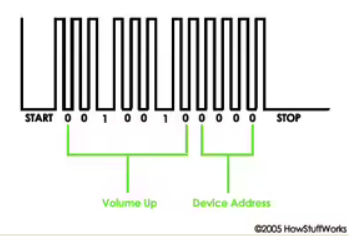
\includegraphics[width=0.9\columnwidth]{./img/buttoncode.png}
  \caption{Example of wave generator for "volume up" from~\cite{btncode})}%
\label{fig:btncode}
\end{figure}

The remote signal includes more than the command for "volume up". It sends several bits of information to the receiving device, including:

-> a "start" command

-> the command code for "volume up"

-> the device address (so the TV knows the data is intended for it)

-> a "stop" command (triggered when you release the "volume up" button)

In this case, the buttons that are needed and its codes are:

Power On = 001 0101

Power Off = 010 1111

Volume Up = 001 0010

Volume Down = 001 0011

